\documentclass[twoside]{article}
\usepackage[a4paper]{geometry}
\geometry{verbose,tmargin=2.5cm,bmargin=2cm,lmargin=2cm,rmargin=2cm}
\usepackage{fancyhdr}
\pagestyle{fancy}

% nastavení pisma a češtiny
\usepackage{lmodern}
\usepackage[T1]{fontenc}
\usepackage[utf8]{inputenc}
\usepackage[czech]{babel}

% odkazy
\usepackage{url}

% vícesloupcové tabulky
\usepackage{multirow}

% vnořené popisky obrázků
\usepackage{subcaption}

% automatická konverze EPS 
\usepackage{graphicx} 
\usepackage{epstopdf}

% odkazy a záložky
\usepackage[unicode=true, bookmarks=true,bookmarksnumbered=true,
bookmarksopen=false, breaklinks=false,pdfborder={0 0 0},
pdfpagemode=UseNone,backref=false,colorlinks=true] {hyperref}

% Poznámky při překladu
\usepackage{xkeyval}	% Inline todonotes
\usepackage[textsize = footnotesize]{todonotes}
\presetkeys{todonotes}{inline}{}

% Zacni sekci slovem ukol
\renewcommand{\thesection}{Úkol \arabic{section}}
% enumerate zacina s pismenem
\renewcommand{\theenumi}{\alph{enumi}}

% smaz aktualni page layout
\fancyhf{}
% zahlavi
\usepackage{titling}
\fancyhf[HC]{\thetitle}
\fancyhf[HLE,HRO]{\theauthor}
\fancyhf[HRE,HLO]{\today}
 %zapati
\fancyhf[FLE,FRO]{\thepage}

% údaje o autorovi
\title{Domácí úkol ARI x}
\author{Vojtěch Michal}
\date{\today}

\begin{document}

\maketitle

% ---------------------------------
% ---------------------------------
% název sekce je generován automaticky jako: Úkol X
\section{~}
\label{sec:ukol1}

\begin{itemize}
\item Otestovat češtinu
\item Napsat rovnici
\item Vložit obrázek
\item Vytvořit tabulku
\item Vyzkoušet odkazy
\end{itemize}

% ---------------------------------
\subsection{~}
\label{sec:Cz}
Schválně jestli schroustne tohle...
\begin{verbatim}
	Příliš žluťoučký kůň úpěl ďábelské ódy.
\end{verbatim}

% ---------------------------------
\subsection{~}
Číslovaná rovnice?
\label{sec:Eq}
\begin{equation}
e^{i \pi} + 1 = 0
\label{eq:TheMostFamousFormula}
\end{equation}

% ---------------------------------
\subsection{~}
\label{sec:Img}
Vektorový obrázek versus jpeg?

\begin{figure}[htb]
	\centering
	\begin{subfigure}[b]{0.45\textwidth}
		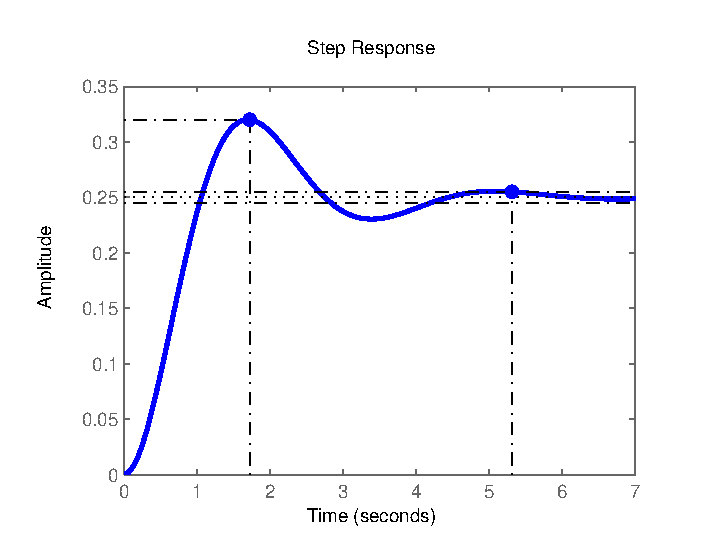
\includegraphics[width=\textwidth]{Figs/StepResponseEPS}
		\caption{Eps obrázek}
		\label{fig:EpsImg}
	\end{subfigure}%
	~ %add desired spacing between images, e. g. ~, \quad, \qquad etc.
	  %(or a blank line to force the subfigure onto a new line)
	\begin{subfigure}[b]{0.45\textwidth}
		\includegraphics[width=\textwidth]{Figs/StepResponseJPG}
		\caption{JPG obrázek (fuj!)}
		\label{fig:JpgImg}
	\end{subfigure}
	\caption{Srovnání kvality *.eps a *.jpg obrázků vložených do \LaTeX.}
	\label{fig:JpgEpsCompare}
\end{figure}

\newpage{}

% ---------------------------------
\subsection{~}
Tabulka s ECTS. Letos určitě budeme lepší!
\label{sec:Tab}
\begin{table}[htb]%
\centering
\begin{tabular}{c|c|c|c}
Známka & ECTS (\%) & 2013 (\%) & 2014 (\%)\\
\hline
A 	& 10 	& 17 	& 50\\
B 	& 25 	& 19 	& 30\\
C 	& 30 	& 22 	& 15\\
D 	& 25 	& 22 	& 5\\
E 	& 10 	& 11 	& 0	\\
F 	& 0 	& 4 	& 0	\\
DNF	& 0 	& 5 	& 0
\end{tabular}
\caption{Statistiky předmětu ARI}
\label{tab:AriStats}
\end{table}

% ---------------------------------
\subsection{~}
\label{sec:Ref}
Odkazy na:
\begin{itemize}
	\item Kapitolu: V kapitole~\ref{tab:AriStats} lze najít statistiky loňského kurzu ARI.
	\item Rovnici: Eulerova rovnost~\ref{eq:TheMostFamousFormula} je 2. nejkrásnější matematický vzorec na světě.
	\item Obrázek: Na Obr.~\ref{fig:JpgEpsCompare} jsou porovnány importované *.eps a *.jpg soubory.
	\item Tabulku: Srovnání úspěšnosti studentů ARI je uvedeno v Tabulce~\ref{tab:AriStats}.
	\item Literaturu: Z videa~\cite{ARI11} přímo čiší nadšení studentů pro tento předmět.
\end{itemize}
Více informací o \LaTeX \ hledejte na stránkách~\cite{Wiki}.


% ---------------------------------
% ---------------------------------
\section{~}
\label{sec:ukol2}
\todo{Absolvovat ARI \cite{ARI11} :-)}


% ---------------------------------
% ---------------------------------
% Literatura
\begin{thebibliography}{9}

% vzorová citace
\bibitem{lamport94}
  Leslie Lamport,
  \emph{\LaTeX: A Document Preparation System}.
  Addison Wesley, Massachusetts,
  2nd Edition,
  1994.

\bibitem{Wiki}
	\LaTeX tutorials, \url{http://en.wikibooks.org/wiki/LaTeX/}

\bibitem{ARI11}
	Studenti předmětu ARI 2011, \emph{ARI song (videoklip)} \url{http://www.youtube.com/watch?v=5gDfQK7dD7c}
\end{thebibliography}












\end{document}

